\section{Motivating Prices}

While \(\bar{X}_n\) is great to build intuition about societies of people, all
its elements are \(n\)-th portions of some total production vector \(x\in X\).
This suggests that everyone would consume the exact same things. And while
clones are great and all, that is not what we are interested in. So how could
multiple people share the goods they produced, without necessarily consuming the
exact same things? 

To satisfy the ``Pluralism in Economics'' crowd, let us avoid
the term ownership for now. We simply observe that some people will produce
things and not necessarily the same people will consume\footnote{
	You can turn a product you can use \(m\) times (before it breaks down)
	without loss of generality into a consumable, by considering these \(m\) uses
	to be individual products. So a person does not ``have'' a chair, but rather
	the \(i\)-th usage of said chair. With this trick in mind, all products are
	consumable.
} the products.
No matter how you organize a society, from an individual perspective, there
are going to be goods the individual \(i\) produces \(S_i\in\real^\dims\) and
goods the individual consumes \(D_i\in\real^\dims\). And fundamentally a
society cannot consume more than is produced (and probably does not want to
produce more than necessary), so we need
\[
	S = \sum_{i=1}^n S_i = \sum_{i=1}^n D_i = D.
\]
The big question is: how can we ensure this? We also want everyone to
voluntarily participate in society. And people are going to stop doing so, if
they feel ripped off as they contribute much more than they get back.
Unfortunately it is difficult to compare the size of two vectors \(S_i\) and
\(D_i\) of uncomparable products. Of course we could enforce \(S_i=D_i\), but
then we are back to hermits, since everyone is using only what they produce.

To make the products comparable again, we could measure them by the time it took
to produce them. But the time needed to produce good \(j\), \(l_i^{(j)}\), might
be different for every person \(i\). Additionally this time is private
information of person \(i\). Especially if we generalize it to be a discomfort
measure instead of strictly time.


\begin{example}[Definitely not Capitalism]
	\label{ex: Definitely not Capitalism}
	Let us try to build a communist utopia, without money and ownership.  For
	this assume that the person which produces good \(j\) jots down their
	subjective cost of production \(l_i^{(j)}\) and tags the product with it and
	puts it into a communal holding space. Additionally they add the cost to
	their ``work-time'' tally.  Whenever someone wants to consume the product,
	they add the cost to their ``consumption-time'' tally, and take the product
	from communal holding space.  Everyone makes sure that their ``work-time''
	tally is comparable to their ``consumption-time''. We have tags, because
	people are bad at estimating how much effort is behind the products they
	consume.

	Does this sound like a utopia? Great!
	We can simplify the two tallies into one, because we only want to make
	sure that the difference is approximately zero. So we might as well add
	``work-time'' and subtract ``consumption-time'' from the get go. We also do not
	need to know how the current tally came to be, so we only need to keep track
	of the running total. This total is going to fluctuate around zero. When it
	is positive, you have worked more for society than you have consumed. And
	vice versa when it is negative.

	Now consider the life of a single product. When it is consumed, the cost was
	added to the tally of the producer and subtracted from the consumer. If you
	had chips to represent the tally, then they would have been simply passed from
	the consumer to the producer. Oh, wait! That's money! People are trading goods
	for money!

	Although right now, tallies can be negative and we do not have negative
	chips/money. This is a problem if you start out with everyone at zero. Because
	nobody can go below that. Or can they? If Alice signs a piece of paper saying
	she owes \(x\) amount of work-time, then she can pass that for a product that
	costs \(x\). The person receiving this note could then pass this note on to
	pay for something too. And if everyone trusts Alice, this is going to go
	swimmingly. So in principle anyone can create money. Money is just the debt
	of someone. The difficulty is creating debt which is widely accepted.

	The balance on a bill splitting app is money (in your friends circle), a coupon
	is money (scammers like to be paid in it), etc. But the money which is most
	widely accepted, is the money issued by a trusted government. Because money is
	debt, so the question whether you accept is, is whether you trust the debtor.
\end{example}
\begin{remark}
	Example~\ref{ex: Definitely not Capitalism} is supposed to show how difficult
	it is to come up with a system which balances production and consumption,
	which is not mathematically equivalent to a market economy. And while the
	initially proposed tally system might be mathematically equivalent, it is
	much less robust and efficient in reality. Because you need to \emph{trust}
	people to update their tallies accurately, \emph{trust} that they make sure
	they don't go too far into the negative, and you need to travel to a
	communal holding space instead of conducting exchanges \emph{decentrally}.
\end{remark}

In the hopes that we justified ownership, trade and prices sufficiently, let us
consider this in more detail. We have suggested using \(l^{(j)}_i\) as prices.
This implies that one good \(j\) has different prices, depending on the producer
\(i\). Since we assume that there are no quality differences, people will
obviously buy the cheaper products first. Let \(p_j\) be the largest price for
which good \(j\) is ever sold. Potential producers \(i\) with \(l^{(j)}_i > p_j\)
refrain from producing good \(j\) and focus their attention on other products.

The producers with \(l^{(j)}_i < p_j\) now see, that they could have sold their
goods for more. And since the cost of production \(l^{(j)}_i\) is private
information, they will likely claim that this cost went up a little next time.
I.e. in the long run, only one prices \(p_j\) per good \(j\) is stable.

\subsection{Finding the Right Prices}


The question remains: What is the right price? Should we average the
\(l^{(j)}_i\) somehow?

It turns out, that ensuring supply to be equal to demand
\(S=D\) leaves us with very little choice when it comes to prices anyway.
Let us see what happens for a fixed price vector. We want \(S=D\). This
obviously implies
\begin{equation}
	\label{eq: supply gdp = demand gdp}
	0 =\langle S-D,p\rangle =  \sum_{i=1}^n \langle S_i - D_i, p\rangle
\end{equation}
A market based system on the other hand ensures
\[
	0 = \langle S_i - D_i, p\rangle
	= \underbrace{\langle S_i, p\rangle}_{\text{income}}
	- \underbrace{\langle D_i,p\rangle}_{\text{expenses}}
\]
which is more than sufficient for the sums in Equation~\eqref{eq: supply gdp =
demand gdp} to be equal, but not sufficient for \(S=D\). In fact, it only
ensures that the price is orthogonal to the demand/supply mismatch \(S-D\).
If there are \(d\) products, that leaves a \(d-1\) hyperplane.

But as we will see, there are some price vectors, which do ensure \(S=D\).
We call these economic equilibria.

\begin{figure}
	\centering
	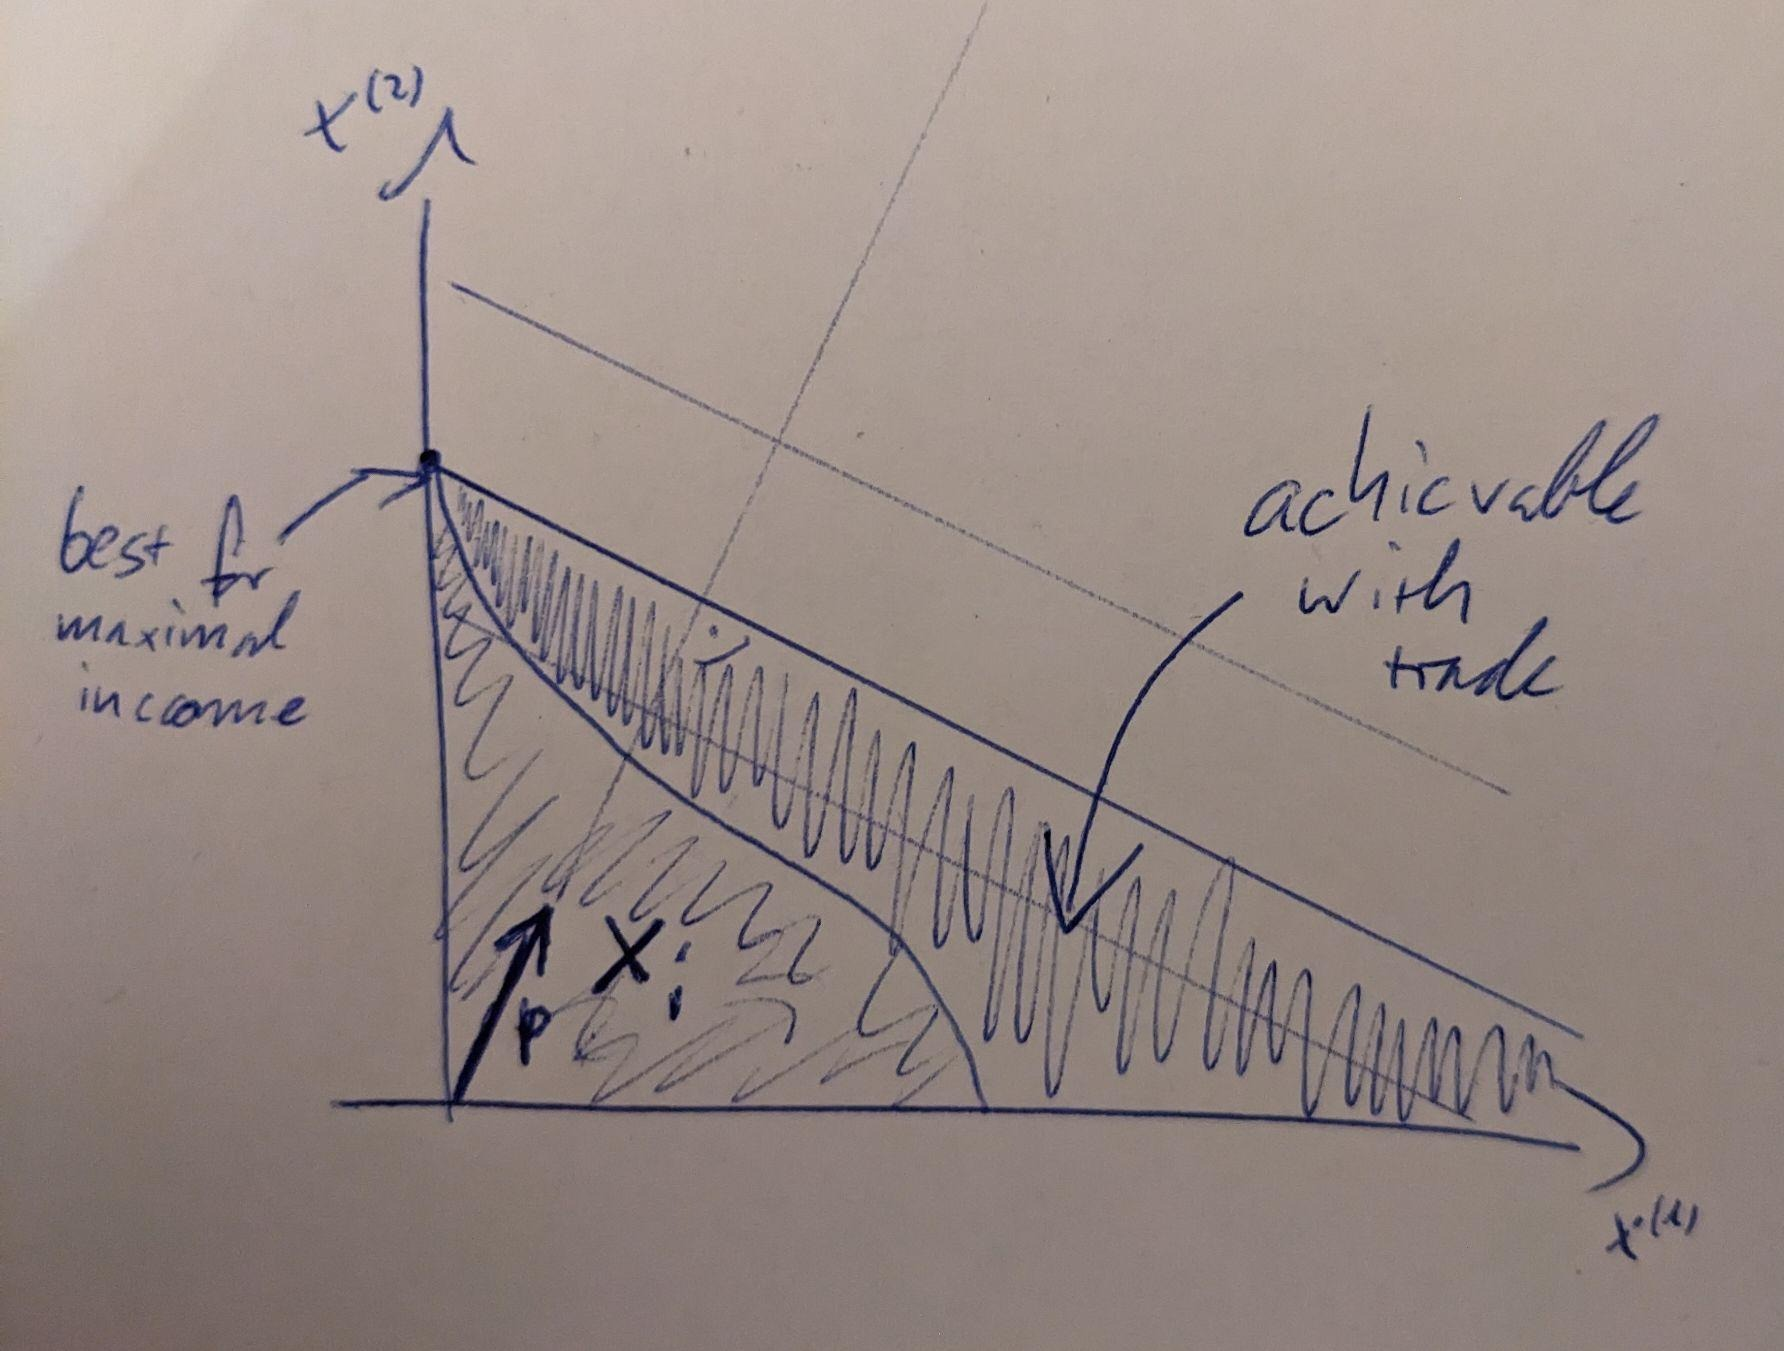
\includegraphics[width=0.7\textwidth]{images/consumption_increase_by_trade.jpeg}
	\caption{
		Product vectors on the \(d-1\) dimensional hyperplanes orthogonal to \(p\)
		cost the same amount and can therefore be exchanged (here \(d=2\), so the
		hyperplanes are lines). Trading at prices \(p\) enlarges the set of
		product vectors available for consumption for person \(i\).
	}
	\label{fig: consumption increase by trade}
\end{figure}
For a fixed price vector \(p\), let us consider the production and consumption
decision of person \(i\). As their expenses have to be smaller than their
income, it makes sense to maximize income for a given amount of labour \(L_i\).
Recall that our production options are \(X_i=X_i(L_i)\). So the maximal income
given labour \(L_i\) is
\[
	\tag{income}\label{eq: income}
	\mu(p, X_i) := \sup\{\langle p, x\rangle : x\in X_i\}.
\]
The function \(\mu(\cdot, X_i)\) in \(p\), is called the ``support function'' of
\(X_i\). It has some useful properties we will be grateful for later on. The
individual decision problem of person \(i\) therefore becomes
\begin{equation}
	\tag{IDP}
	\label{eq: individual decision problem}
	\max_{L_i, y} u(1-L_i, y) \quad\text{subject to}\quad \langle y, p\rangle \le \mu(p, X_i(L_i))
\end{equation}
In Figure~\ref{fig: consumption increase by trade} we can see, how this
constraint is always weaker than \(y\in X_i(L_i)\), which is the constraint of
self-sufficiency. I.e. we get the following lemma.

\begin{lemma}[Trade is never harmful]
\[
	\underbrace{X_i(L_i)}_{\text{own production}}
	\subseteq \quad
	\underbrace{
		\{y\in\real_{\ge 0}^\dims: \langle y, p\rangle \le \mu(p, X_i)\}
	}_{\text{consumption options with trade}}
\]
\end{lemma}
\begin{proof}
	Choose an arbitrary \(y\in X_i\), then by definition of \(\mu\)
	\[
		\langle p, y\rangle \overset{y\in X_i}\le \sup\{\langle p, x\rangle : x\in
		X_i\} \overset{\text{def.}}= \mu(p, X_i),
	\]
	\(y\) is also in the set on the right.
\end{proof}


\begin{lemma}[Income in the Pure Variable Cost Case]
	In the pure variable cost case \(L_i(x) = \langle l_i, x\rangle\), income
	can be written as
	\[
		\mu(p, X_i(L_i))
		= \overbrace{L_i}^{\text{work time}} \max_{j=1,\dots,\dims}
		\underbrace{\frac{p_j}{l_i^{(j)}}}_{=: w_i^{(j)}}
		= L_i \overbrace{\|w_i\|_\infty}^{\text{wage}},
	\]
	where \(w_i^{(j)}\) are potential wages for producing good \(j\).
\end{lemma}
\begin{proof}
	Let \(H:= \diag(l_i)\), then as \(X_i\) is compact we know the supremum is
	a maximum and
	\begin{align*}
		\mu(p, X_i)
		&= \max_{x\ge 0} \langle p, x\rangle
		\text{ s.t. } \langle x, l_i\rangle \le L_i\\
		&\overset{y=Hx}= \max_{y\ge 0} \langle p, H^{-1}y\rangle
		\text{ s.t. } \underbrace{\langle H^{-1}y, l_i\rangle}_{
			= \langle y, 1 \rangle = \|y\|_1
		} \le L_i\\
		&= L_i \underbrace{
			\max_{y\ge 0} \langle H^{-1}p, y\rangle \text{ s.t. } \|y\|_1 \le 1
		}_{
			= \|H^{-1} p\|_{\text{Op-Norm(1)}} = \|H^{-1} p \|_\infty
		}\\
		&= L_i \max_{j=1,\dots,\dims} \frac{p_j}{l_i^{(j)}},
	\end{align*}
	where we have used, that all entries of \(y\) are non-negative when
	converting to the \(1\)-norm, \(\|x\|_1 = \sum_{i=1}^\dims |x_i|\), the
	fact that the operator norm of the \(1\)-norm is the sup norm
	\(\|x\|_\infty = \sup_{i=1,\dots,\dims} |x_i|\)\fxnote{source or appendix},
	and finally positivity of entries of \(p\) and \(l_i\) again.
\end{proof}

\begin{example*}[Pure Variable Cost Case]
	The individual decision problem \eqref{eq: individual decision problem}
	therefore becomes
	\[
		\max_{L_i, y} u(1-L_i, y) \text{ s.t. } \langle p, y\rangle \le L_i \|w_i\|_\infty
	\]
	or in other words
	\[
		\max_{y} u\left(1- \frac{\langle p, y\rangle}{\|w_i\|_\infty}, y\right).
	\]
	The first order condition is therefore
	\[
		\frac{du}{dy} 
		= u_f\Bigl[
			\underbrace{\frac{u_y}{u_f}}_{\text{wtw}}
			- \overbrace{\frac{p}{\|w_i\|_\infty}}^{\text{effort required}}
		\Bigr]
		= \frac{u_f}{\|w_i\|_\infty}\Bigl[
			\underbrace{\frac{u_y}{u_f}\|w_i\|_\infty}_{\text{wtp}}
			- p
		\Bigr]
	\]
	Where the ``willingness to pay'' (wtp) is simply the willingness to work
	(wtw) scaled by person \(i\)'s wages.
	
\end{example*}

\begin{example*}[Pure Variable Cost case with Identical Production Capabilities]

\end{example*}